\documentclass[aspectratio=169,14pt]{beamer}
\usetheme{default}
\usepackage{fontspec}
\setmainfont{texgyrepagella-regular.otf}[BoldFont=texgyrepagella-bold.otf,ItalicFont=texgyrepagella-italic.otf,BoldItalicFont=texgyrepagella-bolditalic.otf]
\setsansfont{texgyreheros-regular.otf}[BoldFont=texgyreheros-bold.otf,ItalicFont=texgyreheros-italic.otf,BoldItalicFont=texgyreheros-bold.otf,BoldItalicFeatures={FakeSlant=0.2}]
\setmonofont{lmmono10-regular.otf}[Scale=0.85]
\setbeamertemplate{navigation symbols}{}
\usepackage{pgfpages}
\newif\ifpresenter
\ifdefined\PresenterVersion\presentertrue\else\presenterfalse\fi
\ifpresenter
  \setbeameroption{show notes on second screen=right}
  \setbeamertemplate{note page}[plain]
\fi
\usepackage{amsmath,amssymb,bm,booktabs,array,graphicx,xcolor}
\usepackage{tikz,pgfplots,adjustbox,listings,xurl}
\pgfplotsset{compat=1.18}
\usetikzlibrary{arrows.meta,positioning,calc,fit,shapes.geometric,decorations.pathreplacing,patterns}
% UIUC official brand colors, verified 2026-10-23.
% https://brand.illinois.edu/visual-identity/color
\definecolor{IlliniOrange}{HTML}{FF5F05}
\definecolor{IlliniBlue}{HTML}{13294B}
\definecolor{Storm}{HTML}{707372}
\definecolor{LightStorm}{HTML}{C6C7C6}
\definecolor{Industrial}{HTML}{1D58A7}
\definecolor{Patina}{HTML}{007E8E}
\tikzset{>=Stealth, every node/.style={font=\small,text=IlliniBlue}, box/.style={draw=IlliniBlue,rounded corners=2pt,align=center,inner sep=6pt,execute at begin node=\hyphenpenalty10000\relax}, orangebox/.style={box,draw=IlliniOrange,very thick}, edge/.style={->,thick,IlliniBlue}, accent/.style={->,very thick,IlliniOrange}}
\pgfplotsset{every axis/.append style={width=13.5cm,height=6.5cm,axis line style={IlliniBlue},tick label style={font=\small,text=IlliniBlue},label style={font=\small,text=IlliniBlue},legend style={font=\small,draw=none,fill=white},grid style={LightStorm},major grid style={LightStorm},axis lines=left,clip=false}, every axis plot/.append style={thick}}

\definecolor{slidepaper}{RGB}{234,220,201}
\setbeamercolor{background canvas}{bg=slidepaper}
\setbeamercolor{normal text}{fg=IlliniBlue}
\setbeamercolor{frametitle}{fg=IlliniBlue}
\setbeamercolor{title}{fg=IlliniBlue}
\setbeamercolor{item}{fg=IlliniOrange}
\setbeamerfont{frametitle}{size=\large,series=\bfseries}
\setbeamerfont{title}{size=\Large,series=\bfseries}
\setbeamertemplate{itemize item}{\color{IlliniOrange}$\bullet$}
\setbeamertemplate{itemize subitem}{\color{IlliniOrange}\footnotesize$\circ$}
\setbeamercolor{orangerule}{bg=IlliniOrange}
\setbeamertemplate{headline}{\begin{beamercolorbox}[wd=\paperwidth,ht=0.1cm,dp=0.1cm]{orangerule}\end{beamercolorbox}}
\setbeamertemplate{footline}{\begin{beamercolorbox}[wd=\paperwidth,ht=0.1cm,dp=0.1cm]{orangerule}\end{beamercolorbox}}
\setbeamersize{text margin left=0.65cm,text margin right=0.65cm}
\setlength{\leftmargini}{1.1em}
\newenvironment{slidebullets}{\begin{itemize}\setlength\itemsep{0.8em}}{\end{itemize}}
\pgfplotsset{every axis/.append style={legend style={fill=slidepaper}}}
\lstdefinelanguage{CoursePython}{keywords={from,import,for,in,if,else,def,return,assert,True,False,None},sensitive=true,morecomment=[l]{\#},morestring=[b]',morestring=[b]"}
\lstset{language=CoursePython,basicstyle=\ttfamily\small,keywordstyle=\color{IlliniBlue}\bfseries,commentstyle=\color{Storm},stringstyle=\color{IlliniBlue},showstringspaces=false,breaklines=true,columns=fullflexible,keepspaces=true,frame=none,aboveskip=0.7em,belowskip=0.7em}
\newcommand{\E}{\mathbb E}
\newcommand{\Var}{\operatorname{Var}}
\newcommand{\Cov}{\operatorname{Cov}}
\hypersetup{colorlinks=true,urlcolor=IlliniBlue,linkcolor=IlliniBlue}

\title{Marketing Analytics}
\subtitle{Text, Social Media, and Networks}
\author{By Nathan Yang}
\date{Session 07}
\begin{document}
\begin{frame}
\titlepage
\end{frame}
\begin{frame}{A Customer-Service Decision}
\usebeamercolor[fg]{normal text}
\vfill
\begin{slidebullets}
\item A retailer wants to detect delivery complaints quickly.
\item The document may be a review, sentence, or service conversation.
\item The action is a review queue with limited staff capacity.
\end{slidebullets}
\vfill
\note{The unit and label definition determine the evaluation. A negative review can concern price or quality rather than delivery. A classifier needs a construct that matches the service action.

M5, Section 5.1, Marketing Analytics Lecture Notes. \url{../06_Lecture_Notes/modules/M05_Text_Social_and_Network_Analysis.md}}
\end{frame}
\begin{frame}{Text Preparation}
\usebeamercolor[fg]{normal text}
\vfill
\begin{slidebullets}
\item Keep negation and domain-specific terms when they affect meaning.
\item Document language, duplicates, and boilerplate.
\item Fit the vocabulary on training documents.
\end{slidebullets}
\vfill
\note{Removing the word not can reverse a sentiment label. Duplicate descriptions across train and test can produce a favorable score for a task requiring generalization to new text.

M5, Section 5.2, Marketing Analytics Lecture Notes. \url{../06_Lecture_Notes/modules/M05_Text_Social_and_Network_Analysis.md}}
\end{frame}
\begin{frame}{TF-IDF Representation}
\usebeamercolor[fg]{normal text}
\noindent Weight a term by frequency in a document and rarity across documents.
\medskip
\[
\operatorname{tfidf}_{td}=\operatorname{tf}_{td}\log\!\left(\frac{N}{\operatorname{df}_t}\right)
\]
\medskip
\noindent Tokenization, smoothing, and normalization are implementation choices that need a record.
\note{Different packages use different conventions. A rare word can be predictive without being substantively important. The vocabulary and IDF values must be learned from the training corpus.

M5, Section 5.2, Marketing Analytics Lecture Notes. \url{../06_Lecture_Notes/modules/M05_Text_Social_and_Network_Analysis.md}}
\end{frame}
\begin{frame}{Embeddings and Similarity}
\usebeamercolor[fg]{normal text}
\vfill
\begin{slidebullets}
\item Embeddings place text in a numerical representation.
\item Nearby descriptions may share meaning or usage.
\item A useful similarity measure still requires domain validation.
\end{slidebullets}
\vfill
\note{A semantic model can confuse closely related foods that have distinct nutritional properties. A cosine score is a representation-based similarity, not a probability of label correctness.

M5, Section 5.3, Marketing Analytics Lecture Notes. \url{../06_Lecture_Notes/modules/M05_Text_Social_and_Network_Analysis.md}}
\end{frame}
\begin{frame}{Labels, Sentiment, and Topics}
\usebeamercolor[fg]{normal text}
\vfill
\begin{slidebullets}
\item Sentiment measures an evaluative construct.
\item Aspect labels distinguish the object of a complaint.
\item Topics summarize recurring term patterns under a model.
\end{slidebullets}
\vfill
\note{A high-weight topic term does not establish a causal driver of satisfaction. Topic names are interpretations that should be checked against representative documents.

M5, Section 5.4, Marketing Analytics Lecture Notes. \url{../06_Lecture_Notes/modules/M05_Text_Social_and_Network_Analysis.md}}
\end{frame}
\begin{frame}{Rare Complaints Lower Precision}
\usebeamercolor[fg]{normal text}
\centering
\begingroup
\begin{adjustbox}{max width=0.98\textwidth,max totalheight=0.65\textheight}
% Original synthetic teaching figure; see corresponding module.
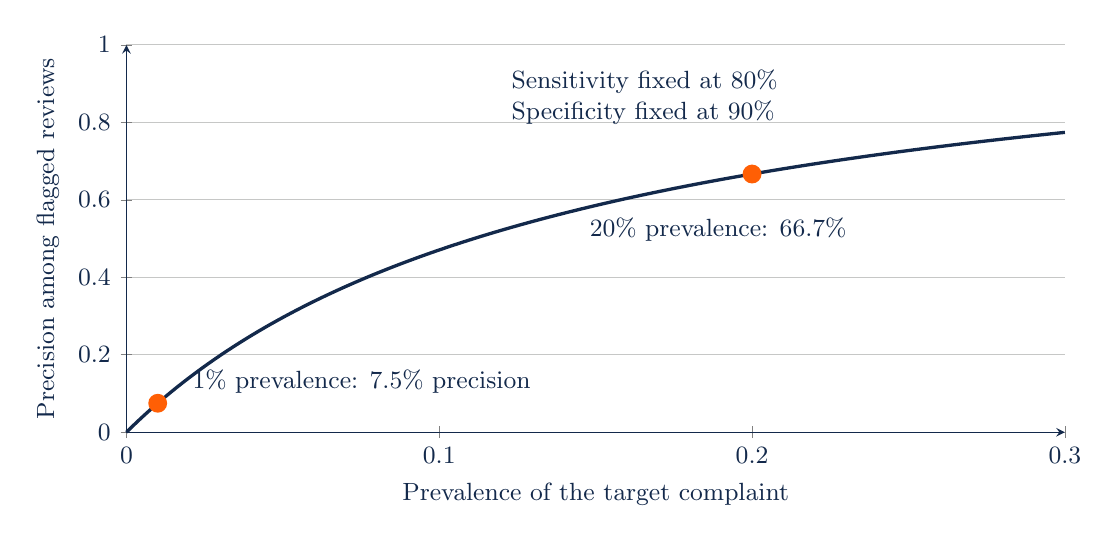
\begin{tikzpicture}
\begin{axis}[xmin=0,xmax=.3,ymin=0,ymax=1,xlabel={Prevalence of the target complaint},ylabel={Precision among flagged reviews},xtick={0,.1,.2,.3},ytick={0,.2,.4,.6,.8,1},ymajorgrids=true]
\addplot[IlliniBlue,very thick,domain=0:.3,samples=150] {.8*x/(.8*x+.1*(1-x))};
\addplot[IlliniOrange,only marks,mark=*,mark size=3pt] coordinates {(.01,.0747664)(.2,.6666667)};
\node[align=left,anchor=north west] at (axis cs:.12,.96) {Sensitivity fixed at 80\%\\Specificity fixed at 90\%};
\node[anchor=west] at (axis cs:.018,.13) {1\% prevalence: 7.5\% precision};
\node[anchor=north west] at (axis cs:.145,.58) {20\% prevalence: 66.7\%};
\end{axis}
\end{tikzpicture}

\end{adjustbox}
\endgroup
\par\medskip
{\small Synthetic classifier. Sensitivity is 80\% and specificity is 90\%.\par}
\note{The classifier has unchanged conditional error rates. The changing base rate alters the composition of the flagged group and therefore the workload of human reviewers.

M5, Section 5.5, Marketing Analytics Lecture Notes. \url{../06_Lecture_Notes/modules/M05_Text_Social_and_Network_Analysis.md}}
\end{frame}
\begin{frame}{Precision Depends on Prevalence}
\usebeamercolor[fg]{normal text}
\noindent Let $\pi$ be complaint prevalence, $s$ sensitivity, and $c$ specificity.
\medskip
\[
\Pr(Y=1\mid\widehat Y=1)=\frac{s\pi}{s\pi+(1-c)(1-\pi)}
\]
\medskip
\noindent False positives can dominate a queue when the target condition is rare.
\note{The formula applies to the specified population and classifier. Prevalence should come from an appropriate deployment sample rather than an artificially balanced training set.

M5, Section 5.5, Marketing Analytics Lecture Notes. \url{../06_Lecture_Notes/modules/M05_Text_Social_and_Network_Analysis.md}}
\end{frame}
\begin{frame}[fragile]{Expected Queue Composition}
\usebeamercolor[fg]{normal text}
\noindent In 10,000 synthetic reviews, complaint prevalence is 1\%.
\begin{lstlisting}
n, prevalence = 10000, 0.01
sensitivity, specificity = 0.8, 0.9
tp = n * prevalence * sensitivity
fp = n * (1-prevalence) * (1-specificity)
precision = tp / (tp + fp)
assert round(precision, 4) == 0.0748
\end{lstlisting}
{\small The expected queue contains 80 true complaints and 990 false positives.\par}
\note{These are expected counts under the imposed rates. Actual counts vary. Capacity planning should consider the queue size as well as sensitivity.

M5, Section 5.5, Marketing Analytics Lecture Notes. \url{../06_Lecture_Notes/modules/M05_Text_Social_and_Network_Analysis.md}}
\end{frame}
\begin{frame}{Human and LLM Annotation}
\usebeamercolor[fg]{normal text}
\vfill
\begin{slidebullets}
\item Write a label definition with difficult boundary examples.
\item Measure agreement and adjudicate disagreements.
\item Assess a held-out sample with human labels.
\item Record the model, prompt, and response format.
\end{slidebullets}
\vfill
\note{Agreement measures consistency, not necessarily construct validity. When a model labels the data used to evaluate itself, the resulting score can reproduce its own labeling choices. A sponsor-framing comparison can hold the same proposal fixed while varying whether the sponsor likes it. Evaluate factual criticism separately from approval. This is a proposed exercise motivated by Sharma et al.; no course model responses have been collected.

M5, Section 5.6, Marketing Analytics Lecture Notes. \url{../06_Lecture_Notes/modules/M05_Text_Social_and_Network_Analysis.md} Sharma et al. (2024), \url{https://arxiv.org/abs/2310.13548v4.} M5 §5.18.}
\end{frame}
\begin{frame}{Agency Labels Need Supporting Evidence}
\usebeamercolor[fg]{normal text}
\vfill
\begin{slidebullets}
\item Extract the outcome, mechanism, study design, and supporting passage.
\item Separate reported choice concerns from inferred possible misuse.
\item Retain uncertain cases and compare independent coding.
\end{slidebullets}
\vfill
\note{Consumer agency concerns understanding, choice, action, and revision or exit. Persuasion alone does not establish impairment. The current literature codes are preliminary AI-assisted annotations without independent human adjudication. Immersive Service supplies qualitative agency evidence; Nudging App Adoption supplies evidence about choice presentation whose misuse requires an additional inference. See M5 Section 5.16.

\url{../03_Data_and_Code/Consumer_Agency_Literature/README.md}}
\end{frame}
\begin{frame}{mHealth Food Descriptions}
\usebeamercolor[fg]{normal text}
\vfill
\begin{slidebullets}
\item Descriptions can recur across many users and dates.
\item A repeated-description split evaluates familiar language.
\item A held-out-description split tests generalization to new language.
\end{slidebullets}
\vfill
\note{The source category is an imperfect label. The same normalized description can have multiple source labels. Evaluation should retain that ambiguity rather than assume a single validated nutrition category.

M5, Section 5.10, Marketing Analytics Lecture Notes. \url{../06_Lecture_Notes/modules/M05_Text_Social_and_Network_Analysis.md}}
\end{frame}
\begin{frame}{Familiar and New Text Are Different Tests}
\usebeamercolor[fg]{normal text}
\centering
\begingroup
\begin{adjustbox}{max width=0.98\textwidth,max totalheight=0.65\textheight}
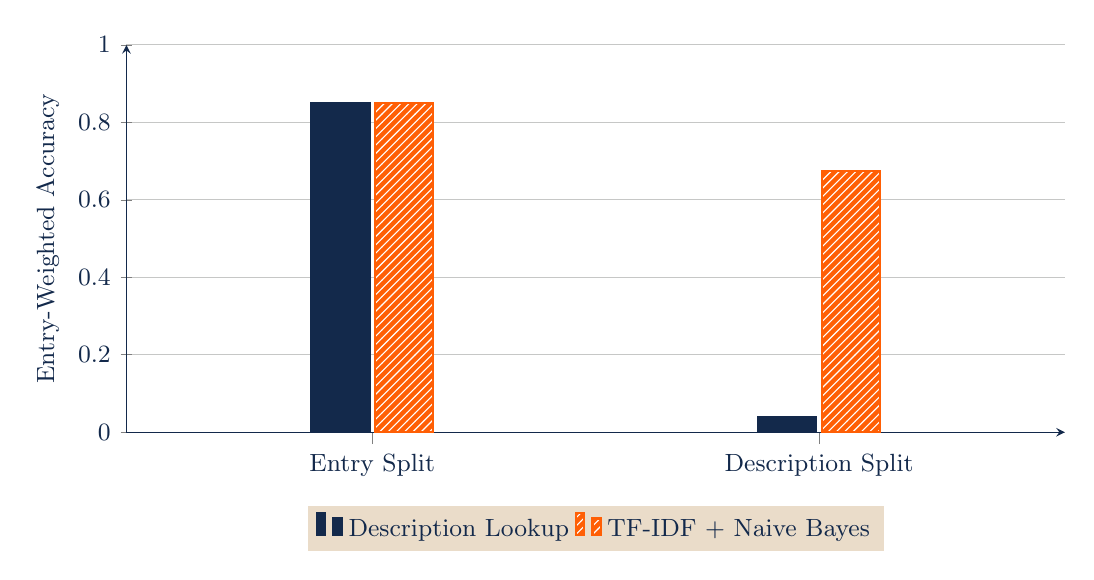
\begin{tikzpicture}
\begin{axis}[ybar,bar width=21pt,ymin=0,ymax=1,ylabel={Entry-Weighted Accuracy},symbolic x coords={Entry Split,Description Split},xtick=data,enlarge x limits=.55,legend style={at={(.5,-.19)},anchor=north,legend columns=2},ymajorgrids=true]
\addplot[fill=IlliniBlue,draw=IlliniBlue] coordinates {(Entry Split,.848956)(Description Split,.038176)};
\addplot[fill=IlliniOrange,draw=IlliniOrange,postaction={pattern=north east lines,pattern color=white}] coordinates {(Entry Split,.849378)(Description Split,.674183)};
\legend{Description Lookup,TF-IDF + Naive Bayes}
\end{axis}
\end{tikzpicture}

\end{adjustbox}
\endgroup
\par\medskip
{\small mHealth text classification uses the stated training and evaluation splits.\par}
\note{A random event split can place an identical description in both training and test. That may be useful for repeated lookup but overstate performance on new descriptions.

M5, Section 5.10, Marketing Analytics Lecture Notes. \url{../06_Lecture_Notes/modules/M05_Text_Social_and_Network_Analysis.md}}
\end{frame}
\begin{frame}{Topic Shares Need a Denominator}
\usebeamercolor[fg]{normal text}
\centering
\begingroup
\begin{adjustbox}{max width=0.98\textwidth,max totalheight=0.65\textheight}
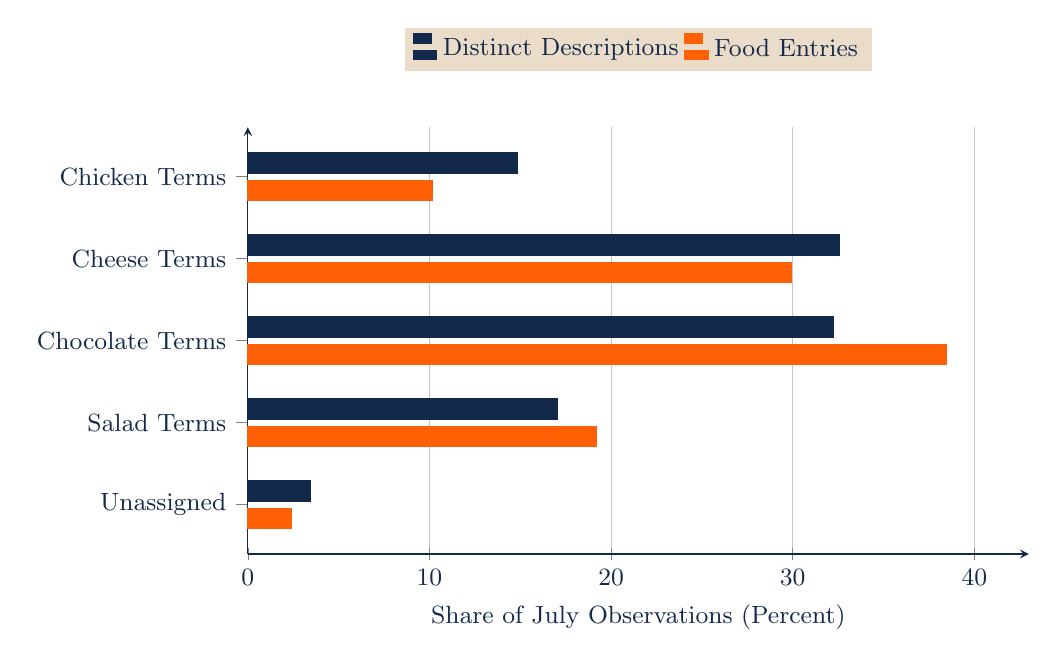
\begin{tikzpicture}
\begin{axis}[xbar,bar width=7pt,width=11.5cm,height=7cm,xlabel={Share of July Observations (Percent)},xmin=0,xmax=43,ymin=-.6,ymax=4.6,ytick={0,1,2,3,4},yticklabels={Unassigned,Salad Terms,Chocolate Terms,Cheese Terms,Chicken Terms},xtick={0,10,20,30,40},xmajorgrids=true,legend style={at={(.5,1.13)},anchor=south,legend columns=2}]
\addplot[IlliniBlue,fill=IlliniBlue,bar shift=5pt] coordinates {(14.833940,4) (32.519657,3) (32.220397,2) (17.005046,1) (3.420960,0)};
\addlegendentry{Distinct Descriptions}
\addplot[IlliniOrange,fill=IlliniOrange,bar shift=-5pt] coordinates {(10.115437,4) (29.924835,3) (38.454419,2) (19.150293,1) (2.355016,0)};
\addlegendentry{Food Entries}
\end{axis}\end{tikzpicture}

\end{adjustbox}
\endgroup
\par\medskip
{\small mHealth topic summaries compare documents, entries, and users under defined weights.\par}
\note{Long documents and repeated records can dominate term-weighted summaries. A business question about the fraction of affected customers needs a customer denominator.

M5, Section 5.12, Marketing Analytics Lecture Notes. \url{../06_Lecture_Notes/modules/M05_Text_Social_and_Network_Analysis.md}}
\end{frame}
\begin{frame}{Which Pricing Statements Deserve Review?}
\usebeamercolor[fg]{normal text}
\vfill
\begin{slidebullets}
\item A retailer reviews competitors' public pricing communication.
\item A keyword occurrence supplies a reading lead.
\item Define the priced object, timing, and evidence before interpreting adoption.
\end{slidebullets}
\vfill
\note{The supplied corpus includes core terms for pricing methods and shelf-label infrastructure. Among observed calls, core-call rates are 2.90\% in retail, 2.02\% in restaurants, and 10.49\% in the selected comparison group. These are call-weighted disclosure rates.

M5, Section 5.14, Marketing Analytics Lecture Notes. \url{../06_Lecture_Notes/modules/M05_Text_Social_and_Network_Analysis.md}}
\end{frame}
\begin{frame}{Speaking Time Changes the Comparison}
\usebeamercolor[fg]{normal text}
\centering
\begingroup
\begin{adjustbox}{max width=0.98\textwidth,max totalheight=0.65\textheight}
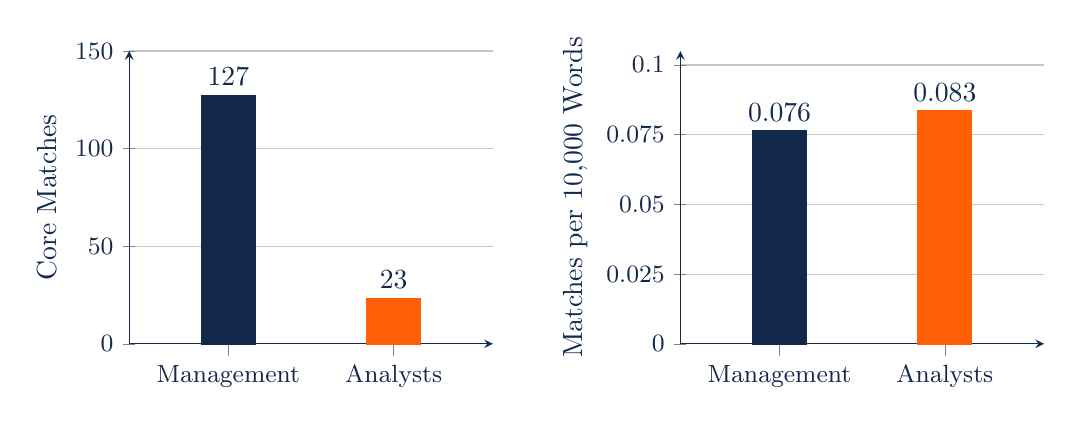
\begin{tikzpicture}
\begin{axis}[at={(0cm,0)},anchor=south west,width=6.2cm,height=5.3cm,
 ybar,bar shift=0pt,bar width=19pt,xmin=-.6,xmax=1.6,ymin=0,ymax=150,
 xtick={0,1},xticklabels={Management,Analysts},ytick={0,50,100,150},
 ylabel={Core Matches},ymajorgrids=true,nodes near coords,
 tick label style={font=\fontsize{9}{11}\selectfont},
 label style={font=\fontsize{10}{12}\selectfont},
 yticklabel style={/pgf/number format/fixed,/pgf/number format/precision=3},
 every node near coord/.append style={font=\fontsize{10}{12}\selectfont},
 point meta=explicit symbolic]
\addplot[fill=IlliniBlue,draw=IlliniBlue] coordinates {(0,127) [127]};
\addplot[fill=IlliniOrange,draw=IlliniOrange] coordinates {(1,23) [23]};
\end{axis}
\begin{axis}[at={(7cm,0)},anchor=south west,width=6.2cm,height=5.3cm,
 ybar,bar shift=0pt,bar width=19pt,xmin=-.6,xmax=1.6,ymin=0,ymax=0.105,
 xtick={0,1},xticklabels={Management,Analysts},ytick={0,.025,.05,.075,.1},
 ylabel={Matches per 10,000 Words},ymajorgrids=true,nodes near coords,
 tick label style={font=\fontsize{9}{11}\selectfont},
 label style={font=\fontsize{10}{12}\selectfont},
 yticklabel style={/pgf/number format/fixed,/pgf/number format/precision=3},
 every node near coord/.append style={font=\fontsize{10}{12}\selectfont},
 point meta=explicit symbolic]
\addplot[fill=IlliniBlue,draw=IlliniBlue] coordinates {(0,0.0761147301900626) [0.076]};
\addplot[fill=IlliniOrange,draw=IlliniOrange] coordinates {(1,0.0832730207360683) [0.083]};
\end{axis}
\end{tikzpicture}

\end{adjustbox}
\endgroup
\par\medskip
{\small Observed calls; heuristic roles. Management includes prepared remarks and Q\&A.\par}
\note{Raw counts rank management higher, whereas exposure-adjusted intensity is slightly higher for analysts. This is a descriptive arithmetic comparison, with different formats and heuristic labels. Restricting both counts and words to detected-Q\&A calls gives rates of 0.072 and 0.083.

M5, Section 5.14, Marketing Analytics Lecture Notes. \url{../06_Lecture_Notes/modules/M05_Text_Social_and_Network_Analysis.md}}
\end{frame}
\begin{frame}{Same Vocabulary, Different Evidence}
\usebeamercolor[fg]{normal text}
\vfill
\begin{slidebullets}
\item Amazon: current price information; Eventbrite: advertising cost per click.
\item Wendy's: planned tests; Kroger: shelf-label infrastructure.
\item A claim about use still requires evidence on implementation and outcomes.
\end{slidebullets}
\vfill
\note{Seven purposeful, source-linked paraphrases are provided in interpretation\_cases.csv. They are examples of construct distinctions, not a representative precision sample. Delta's January 2025 question recorded as management/prepared also motivates reviewing heuristic speaker boundaries.

M5, Section 5.14, Marketing Analytics Lecture Notes. \url{../06_Lecture_Notes/modules/M05_Text_Social_and_Network_Analysis.md}}
\end{frame}
\begin{frame}[fragile]{Match Counts and Words to the Same Calls}
\usebeamercolor[fg]{normal text}
\noindent From the Earnings\_Calls folder, compare the verified metadata.
\begin{lstlisting}
from assessment import load_checked
from disclosure import role_rates
calls, mentions, _, _ = load_checked()
rates = role_rates(calls, mentions, require_qa=True)
assert rates.calls.eq(2240).all()
print(rates[['role', 'core_matches', 'per_10000_words']])
\end{lstlisting}
{\small Excluding a call removes both its occurrences and its words.\par}
\note{Run disclosure.py for group, quarterly, and role tables. The counterexample test includes one excluded call with many words; dropping only its matches would change the rate incorrectly.

M5, Section 5.14, Marketing Analytics Lecture Notes. \url{../06_Lecture_Notes/modules/M05_Text_Social_and_Network_Analysis.md}}
\end{frame}
\begin{frame}{Evaluate Retrieval and Interpretation Separately}
\usebeamercolor[fg]{normal text}
\vfill
\begin{slidebullets}
\item A denial and a future intention can match the same phrase.
\item Relevant paraphrases can escape the dictionary.
\item Validate held-out firms or later calls with independently labeled hits and misses.
\end{slidebullets}
\vfill
\note{Run construct\_checks.py for eight synthetic sentences. A purposeful case set cannot estimate corpus precision or recall. Probability sampling and appropriate weights are needed for population metrics. No external model or labeling API was run for the supplied course example.

M5, Section 5.14, Marketing Analytics Lecture Notes. \url{../06_Lecture_Notes/modules/M05_Text_Social_and_Network_Analysis.md}}
\end{frame}
\begin{frame}{Prompt Revision Uses Evaluation Evidence}
\usebeamercolor[fg]{normal text}
\vfill
\begin{slidebullets}
\item A passage used to revise a prompt becomes development material.
\item Keep passages from one call together when constructing a split.
\item Freeze the prompt and reference-label procedure before fresh evaluation.
\end{slidebullets}
\vfill
\note{A test on new firms addresses a different deployment population from a test on later calls from familiar firms. Repeated passages are not independent firm-level replications. Evaluate a competent dictionary baseline with the same eligible evidence. Once final labels guide a revision, a later confirmation needs new evidence or a justified adaptive-evaluation design.

Marketing Analytics Lecture Notes, M5 §5.15.}
\end{frame}
\begin{frame}{Generator and Judge Changes}
\usebeamercolor[fg]{normal text}
\centering
\begingroup
\fontsize{11}{13.2}\selectfont
\def\small{\fontsize{10}{12}\selectfont}
\def\footnotesize{\fontsize{9}{11}\selectfont}
\def\scriptsize{\fontsize{8}{9.5}\selectfont}
\hyphenpenalty=10000
\begin{adjustbox}{max width=0.98\textwidth,max totalheight=0.65\textheight}
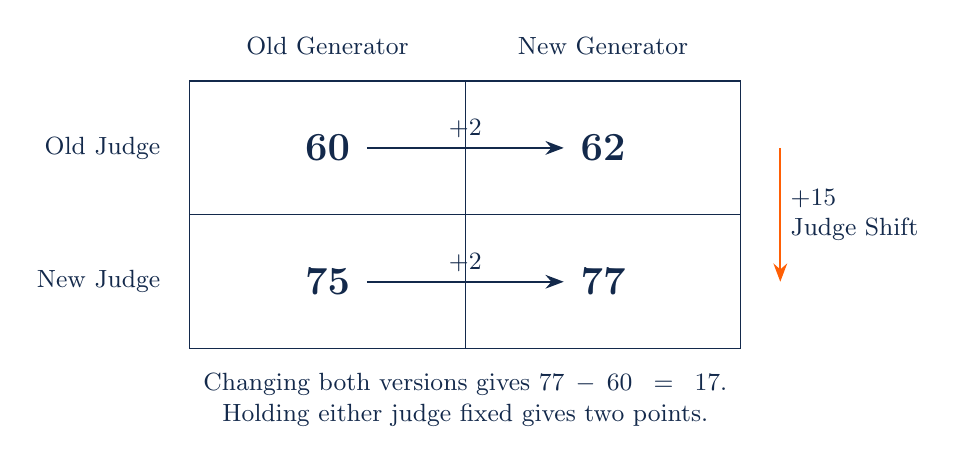
\begin{tikzpicture}[font=\small,>=Stealth]
\draw[IlliniBlue] (0,0) rectangle (7,3.4);
\draw[IlliniBlue] (3.5,0)--(3.5,3.4);
\draw[IlliniBlue] (0,1.7)--(7,1.7);
\node at (1.75,3.85) {Old Generator};
\node at (5.25,3.85) {New Generator};
\node[anchor=east] at (-.25,2.55) {Old Judge};
\node[anchor=east] at (-.25,.85) {New Judge};
\node[font=\Large\bfseries] at (1.75,2.55) {60};
\node[font=\Large\bfseries] at (5.25,2.55) {62};
\node[font=\Large\bfseries] at (1.75,.85) {75};
\node[font=\Large\bfseries] at (5.25,.85) {77};
\draw[->,IlliniBlue,thick] (2.25,2.55)--node[above] {$+2$} (4.75,2.55);
\draw[->,IlliniBlue,thick] (2.25,.85)--node[above] {$+2$} (4.75,.85);
\draw[->,IlliniOrange,thick] (7.5,2.55)--node[right,align=left] {$+15$\\Judge Shift} (7.5,.85);
\node[align=center,text width=9.2cm] at (3.5,-.65) {Changing both versions gives $77-60=17$.\\Holding either judge fixed gives two points.};
\end{tikzpicture}

\end{adjustbox}
\endgroup
\par\medskip
{\small Identical saved outputs are scored by both judges. All scores are stipulated.\par}
\note{A stable judge supplies a common comparison but still requires validation. Position, verbosity, and self-preference can affect evaluation. For earnings-call summaries, independently check factual support, speaker role, and whether a statement concerns a plan or an implemented action. Preserve inconsistent judgments.

M5 §5.18. Zheng et al. (2023), \url{https://arxiv.org/abs/2306.05685;} Panickssery et al. (2024), \url{https://arxiv.org/abs/2404.13076}}
\end{frame}
\begin{frame}{Network Objects}
\usebeamercolor[fg]{normal text}
\vfill
\begin{slidebullets}
\item Nodes identify customers or accounts.
\item Edges represent a defined relationship in a time window.
\item Degree counts links, while brokerage concerns paths between groups.
\end{slidebullets}
\vfill
\note{An edge could mean following, messaging, purchasing together, or co-occurrence. Those meanings are not interchangeable. The network boundary determines which relationships are visible.

M5, Section 5.7, Marketing Analytics Lecture Notes. \url{../06_Lecture_Notes/modules/M05_Text_Social_and_Network_Analysis.md}}
\end{frame}
\begin{frame}{Few Links Can Connect Separate Groups}
\usebeamercolor[fg]{normal text}
\centering
\begingroup
\fontsize{11}{13.2}\selectfont
\def\small{\fontsize{10}{12}\selectfont}
\def\footnotesize{\fontsize{9}{11}\selectfont}
\def\scriptsize{\fontsize{8}{9.5}\selectfont}
\hyphenpenalty=10000
\begin{adjustbox}{max width=0.98\textwidth,max totalheight=0.65\textheight}
% Original synthetic teaching figure; see corresponding module.
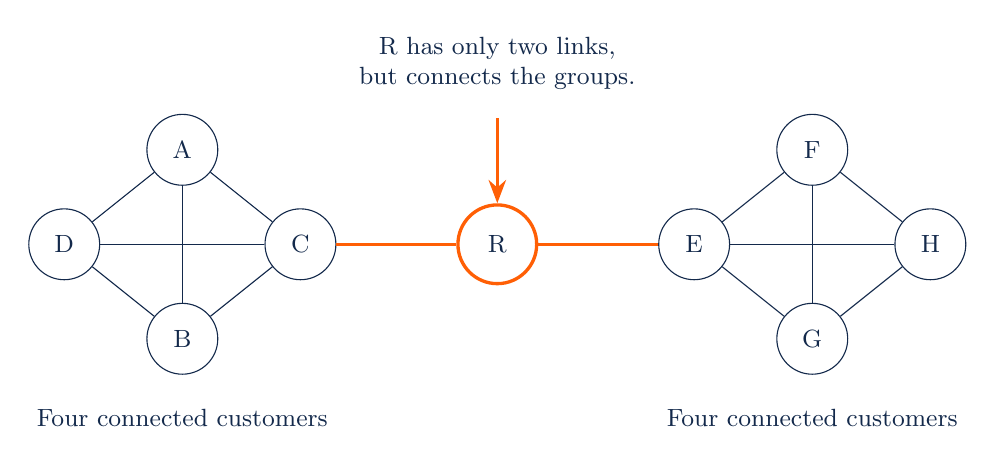
\begin{tikzpicture}[v/.style={circle,draw=IlliniBlue,fill=white,minimum size=9mm},b/.style={circle,draw=IlliniOrange,very thick,fill=white,minimum size=10mm}]
\node[v] (a) at (0,1.2) {A};\node[v] (b) at (0,-1.2) {B};\node[v] (c) at (1.5,0) {C};\node[v] (d) at (-1.5,0) {D};
\node[b] (r) at (4,0) {R};
\node[v] (e) at (6.5,0) {E};\node[v] (f) at (8,1.2) {F};\node[v] (g) at (8,-1.2) {G};\node[v] (h) at (9.5,0) {H};
\foreach \x/\y in {a/b,a/c,a/d,b/c,b/d,c/d,e/f,e/g,e/h,f/g,f/h,g/h} {\draw[IlliniBlue] (\x)--(\y);}
\draw[IlliniOrange,very thick] (c)--(r)--(e);
\node[align=center] at (0,-2.2) {Four connected customers};
\node[align=center] at (8,-2.2) {Four connected customers};
\node[align=center,text width=4cm] at (4,2.3) {R has only two links,\\but connects the groups.};
\draw[accent] (4,1.6)--(r.north);
\end{tikzpicture}

\end{adjustbox}
\endgroup
\par\medskip
{\small Synthetic undirected network. R has only two links.\par}
\note{Brokerage can matter for reach even when a node has few direct neighbors. Observed network structure does not by itself establish the effect of targeting that person.

M5, Section 5.7, Marketing Analytics Lecture Notes. \url{../06_Lecture_Notes/modules/M05_Text_Social_and_Network_Analysis.md}}
\end{frame}
\begin{frame}{University Affiliations Create a Research Network}
\usebeamercolor[fg]{normal text}
\vfill
\begin{slidebullets}
\item 745 papers identify 424 higher-education institutions.
\item Split one unit of link weight across each paper's university pairs.
\item Shared-paper links can also arise from a single author's dual affiliation.
\end{slidebullets}
\vfill
\note{The eligible census has 824 papers; 79 lack identified education affiliations. Work-specific metadata is used rather than current author profiles. One missing University of Vaasa affiliation was verified from a published article and corrected. Louvain clustering at resolution one and seed 534 finds 19 communities among 415 linked institutions; nine remain unconnected. See M5 Section 5.17.

\url{../03_Data_and_Code/Consumer_Agency_Literature/AFFILIATIONS.md}}
\end{frame}
\begin{frame}{Affiliation Groups Depend on the Representation}
\usebeamercolor[fg]{normal text}
\centering
\begingroup
\begin{adjustbox}{max width=0.98\textwidth,max totalheight=0.65\textheight}
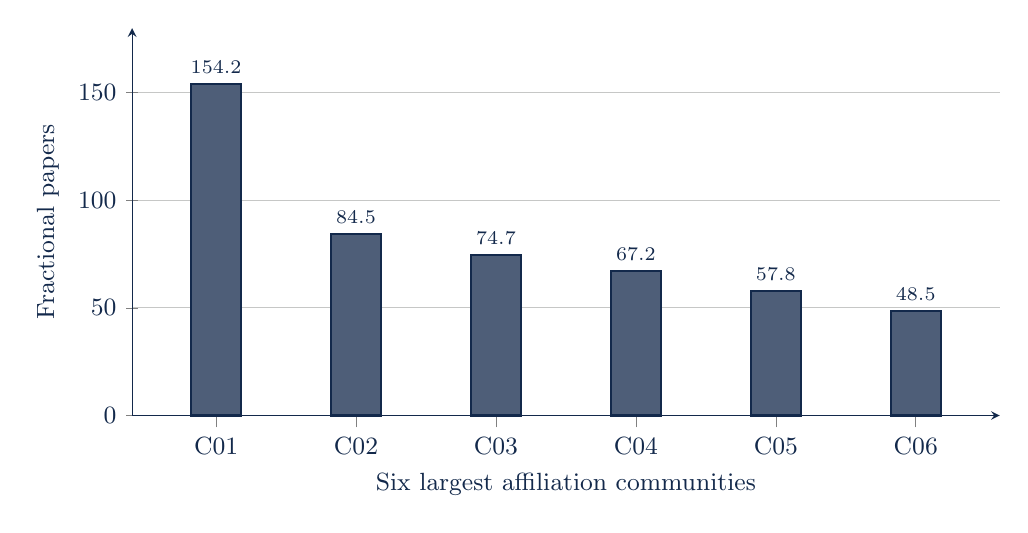
\begin{tikzpicture}
\begin{axis}[
 ybar,width=12.6cm,height=6.5cm,bar width=18pt,
 ymin=0,ymax=180,ytick={0,50,100,150},
 ylabel={Fractional papers},xlabel={Six largest affiliation communities},
 symbolic x coords={C01,C02,C03,C04,C05,C06},xtick=data,
 enlarge x limits=.12,ymajorgrids=true,
 nodes near coords,nodes near coords style={font=\scriptsize},
 every node near coord/.append style={/pgf/number format/fixed,/pgf/number format/precision=1}]
\addplot[fill=IlliniBlue!75,draw=IlliniBlue] coordinates {
(C01,154.15000000) (C02,84.53730159) (C03,74.65396825) (C04,67.16111111) (C05,57.79563492) (C06,48.52261905)};
\end{axis}
\end{tikzpicture}

\end{adjustbox}
\endgroup
\par\medskip
{\small Fractional papers in the six largest of 19 communities. All 745 papers contribute one in total.\par}
\note{The median adjusted Rand agreement across twenty seeds is 0.522; switching from fractional to full edge counting gives 0.193. These are exploratory communities. The selected mechanism overlay has uneven review coverage and cannot establish institutional intent or rank universities by harm. The full program and all memberships appear in M5 Section 5.17 and the affiliation outputs.

\url{../03_Data_and_Code/Consumer_Agency_Literature/AFFILIATIONS.md}}
\end{frame}
\begin{frame}{Coding Exercise: A Label Assessment}
\usebeamercolor[fg]{normal text}
\vfill
\begin{slidebullets}
\item Run the earnings-call assessment and role-exposure calculation.
\item Test denial, future intention, and a missed paraphrase.
\item Explain which extra labels would identify precision and recall.
\end{slidebullets}
\vfill
\note{Use ../03\_Data\_and\_Code/Earnings\_Calls/README.md and LLM\_EXERCISES.md. The mHealth example provides a second application of held-out description evaluation. Synthetic dictionary contrasts are implementation checks; they do not estimate deployment accuracy.

M5, Section 5.9, Marketing Analytics Lecture Notes. \url{../06_Lecture_Notes/modules/M05_Text_Social_and_Network_Analysis.md}}
\end{frame}
\begin{frame}{Engagement and Commercial Value}
\usebeamercolor[fg]{normal text}
\vfill
\begin{slidebullets}
\item Likes and comments measure platform responses.
\item Sales and contribution require separate outcome records.
\item Network similarity can reflect common interests or common exposure.
\end{slidebullets}
\vfill
\note{Homophily and shared shocks can generate correlated behavior among connected users. A causal influence claim requires an assignment or identification design beyond a network correlation.

M5, Section 5.8, Marketing Analytics Lecture Notes. \url{../06_Lecture_Notes/modules/M05_Text_Social_and_Network_Analysis.md}}
\end{frame}
\begin{frame}{Authenticity of Reviews and Endorsements}
\usebeamercolor[fg]{normal text}
\vfill
\begin{slidebullets}
\item A generated product description and a claimed customer review serve different roles.
\item A fabricated experience misrepresents the source of the evidence.
\item Keep sponsored relationships and substantive editing traceable.
\end{slidebullets}
\vfill
\note{The FTC review rule addresses business conduct involving fake or false reviews. Its FAQ distinguishes mere review hosting from creation, purchase, and dissemination of testimonials, with provision-specific conditions.

FTC Consumer Reviews and Testimonials Rule Q\&A. \url{https://www.ftc.gov/business-guidance/resources/consumer-reviews-testimonials-rule-questions-answers}}
\end{frame}
\begin{frame}{Text-Analysis Discussion}
\usebeamercolor[fg]{normal text}
\vfill
\begin{slidebullets}
\item Which label disagreement would change the service decision?
\item How does the expected queue change when prevalence falls?
\item What comparison would distinguish exposure from influence?
\end{slidebullets}
\vfill
\note{A practical assessment prioritizes errors that alter the action. False positives determine review burden, while false negatives determine missed cases. Both should be evaluated in the deployment population.

M5, Section 5.9, Marketing Analytics Lecture Notes. \url{../06_Lecture_Notes/modules/M05_Text_Social_and_Network_Analysis.md}}
\end{frame}
\end{document}
